\documentclass[10pt,twocolumn,letterpaper]{article}

\usepackage{cvpr}
\usepackage{times}
\usepackage{epsfig}
\usepackage{graphicx}
\usepackage{amsmath}
\usepackage{amssymb}
\usepackage{subfig}

% \usepackage{graphicx}
% \usepackage{subfigure}
% \usepackage{xcolor}
% \usepackage{color, soul}


% \renewcommand{\thetable}{S\arabic{table}}

% Include other packages here, before hyperref.

% If you comment hyperref and then uncomment it, you should delete
% egpaper.aux before re-running latex.  (Or just hit 'q' on the first latex
% run, let it finish, and you should be clear).
\usepackage[pagebackref=true,breaklinks=true,letterpaper=true,colorlinks,bookmarks=false]{hyperref}

\cvprfinalcopy % *** Uncomment this line for the final submission

\def\cvprPaperID{****} % *** Enter the CVPR Paper ID here
\def\httilde{\mbox{\tt\raisebox{-.5ex}{\symbol{126}}}}

% Pages are numbered in submission mode, and unnumbered in camera-ready
\ifcvprfinal\pagestyle{empty}\fi

%%%%%%%%% TITLE
\title{A Billion-Dollar Material \\
\large Finding Ultra-Low Emittance Photocathode Materials for Linear Accelerators}

\author{
Michael Cai\\
Department of CS\\
Stanford University\\
{\tt\small mcai88@stanford.edu}
\and
Michael Cooper\\
Department of CS\\
Stanford University\\
{\tt\small coopermj@stanford.edu}
\and
Jennie Yang\\
Department of MSE\\
Stanford University\\
{\tt\small jenniey@stanford.edu}
}

\begin{document}

\twocolumn[{%
\renewcommand\twocolumn[1][]{#1}%
\maketitle
}]

\thispagestyle{empty}

% %%%%%%%%% ABSTRACT
\begin{abstract}
We investigate AI-based approaches for improving computation times of the thermal emittance of photocathode material candidates. We frame the problem as a binary classification problem, describe three standardized approaches for representing material features as inputs for machine learning models, and evaluate the performance of common machine learning models on this task. We conclude that a neural network model based on the average atomic properties for each material is the best performing model, though more advanced data representations could be applied in future to increase prediction accuracy.
\end{abstract}

%%%%%%%%% BODY TEXT
\section{Introduction}

The Stanford Linear Accelerator Center \textbf{(SLAC)} is one of the world's premier tools for studying advanced physics and chemistry. In this project, we explore the application of machine learning to the field of Computational Materials Science to find new materials to satisfy a set of desired properties for SLAC experiments.

A team headed by Associate Professor \textbf{Dr. Evan Reed} of Stanford's Department of Materials Science and Engineering is in the early stages of a project in collaboration with SLAC, the goal of which is to use computational methods to predict materials with sufficiently low \textbf{thermal emittance} to use in advanced photocathodes in particle accelerators. Thermal emittance is inversely proportional to beam brightness, so low-emittance materials enable sensing with the use of more powerful electron beams and, therefore, new experiments.

The Reed Group currently deploys a model based on Density Functional Theory \textbf{(DFT)}, an accurate but computationally expensive method for generating a material's electronic band structure, from which thermal emittance can be easily computed. The DFT model takes anywhere between several hours to a full day to predict the emittance of one candidate material; thus, the goal of our project is to use machine learning on these DFT results in hopes of significantly expediting the prediction process.

%%%%%%%%%%%%%%%%Related Work%%%%%%%%%%%%%%%%%%%%%%%%

%Need to expand more
\section{Related Work}

In 2010, Dowell \textit{et al} proposed a three-part plan of photocathode R\&D: (1) study cathode formation and emission with existing diagnostic strategies, (2) model emission and electron dynamics in cathodes, and (3) test cathodes in operation. \cite{Dowell} 
This plan is consistent with the typical process of  materials research, which centers on studying known (though perhaps poorly-understood) materials and developing physical models to describe them. For example, in accordance with step (1) of this R\&D plan, Bazarov \textit{et al} used a solenoid scan to measure the emittance of a cesium potassium antimonide photocathode. \cite{Bazarov}

While such physical experiments are vital to materials research, they are time-consuming and perform poorly at scale. These techniques are impractical for screening a large quantity of materials or analyzing materials which cannot yet be fabricated. Computational models, on the other hand, allow researchers to study the properties of materials without requiring physical samples. In 2015, Li \textit{et al} explored the connection between the electronic band structure of photocathodes and the momentum of the emitted electrons \cite{Li}, which helped make it possible to determine thermal emittance through DFT. While such computation is faster than physical experimentation, it can still prove too slow for the study of a large quantity of materials. Thus, machine learning may prove a faster early-screening tool to complement computational materials research.

Machine learning in materials science is a new frontier: machine learning-compatible representations of materials is very much an active area of research. For example, in April 2019, Himanen \textit{et al} released DScribe, a software package for generating several different kinds of ML-friendly descriptors of materials, including the Coulomb and Ewald sum matrices. \cite{DScribe} Unfortunately for our purposes, the representations provided by DScribe are best applied when dealing with materials all of the same class; our dataset is too diverse to appropriately apply the DScribe library.

Instead, one of the material-representation methods we use in our investigation is a variant of the "elemental descriptors" method described by Cubuk, \textit{et al}, which is based on the composition of the material rather than its structure \cite{Cubuk}, making it suitable to describe the wide range of materials in our dataset. 


%%%%%%%%%%%%%%%%%%%%%%Data%%%%%%%%%%%%%%%%%%%%%%%%%%%%%%%%%%%%%
\section{Data and Features}

\subsection{Data}
The Reed Lab provided us a list of candidate materials. Of these candidates, 9,436 also have associated emittance data, calculated through a DFT-based approach. Each material's emittance data is represented as a series of 100 emittance values as a function of incident photon energy, starting at the material's band gap energy ($E_g$) and going up to $E_g + 5$ eV. For each material, we extracted our features via the Materials Project API (documented \href{https://materialsproject.org/}{here}) and through the \texttt{mendeleev} Python package (documented \href{https://mendeleev.readthedocs.io/en/latest/index.html}{here}) \cite{mendeleev}.

\subsection{Input Representations}

Representing the materials in our dataset was a significant challenge, as no known representation can fully capture both the physical and structural properties of a material, and work well with both molecular and lattice-based materials. In this project, we evaluated performance on three different data representations.

\subsubsection{Unit Cell Representation}
Our preliminary method of representing each material features a \textbf{71-element vector} encoding the unit cell (smallest repeating unit for a crystal). The first three entries of the vector give the lattice parameters, which are the dimensions of its unit cell ($a$, $b$, $c$), the next three entries are the alpha-beta-gamma angles between the a,b,c axes ($\alpha$, $\beta$, $\gamma$), and the seventh entry gives the relaxed unit cell volume ($v$). See Figure \ref{fig:Unit-Cell} for a visual representation of these parameters. The final 64 entries give the atomic number of each of the first 16 atoms ($e_i$) in the unit cell followed by the locations of each atom in the material as a proportion of each a-b-c dimension ($a_i$, $b_i$, $c_i$). 
$$\Vec{X} = [a, b, c, \alpha, \beta, \gamma, v, e_0, a_0, b_0, c_0, ..., e_{15}, a_{15}, b_{15}, c_{15}]$$
For non-crystalline materials, the unit cell is set such that it contains one molecule of the material. All of our unit cell information for both crystalline and non-crystalline materials is drawn from the Materials Project's database. Unused entries in each feature vector are zero-padded to standardize input length. 


\begin{figure}[ht]
\centering
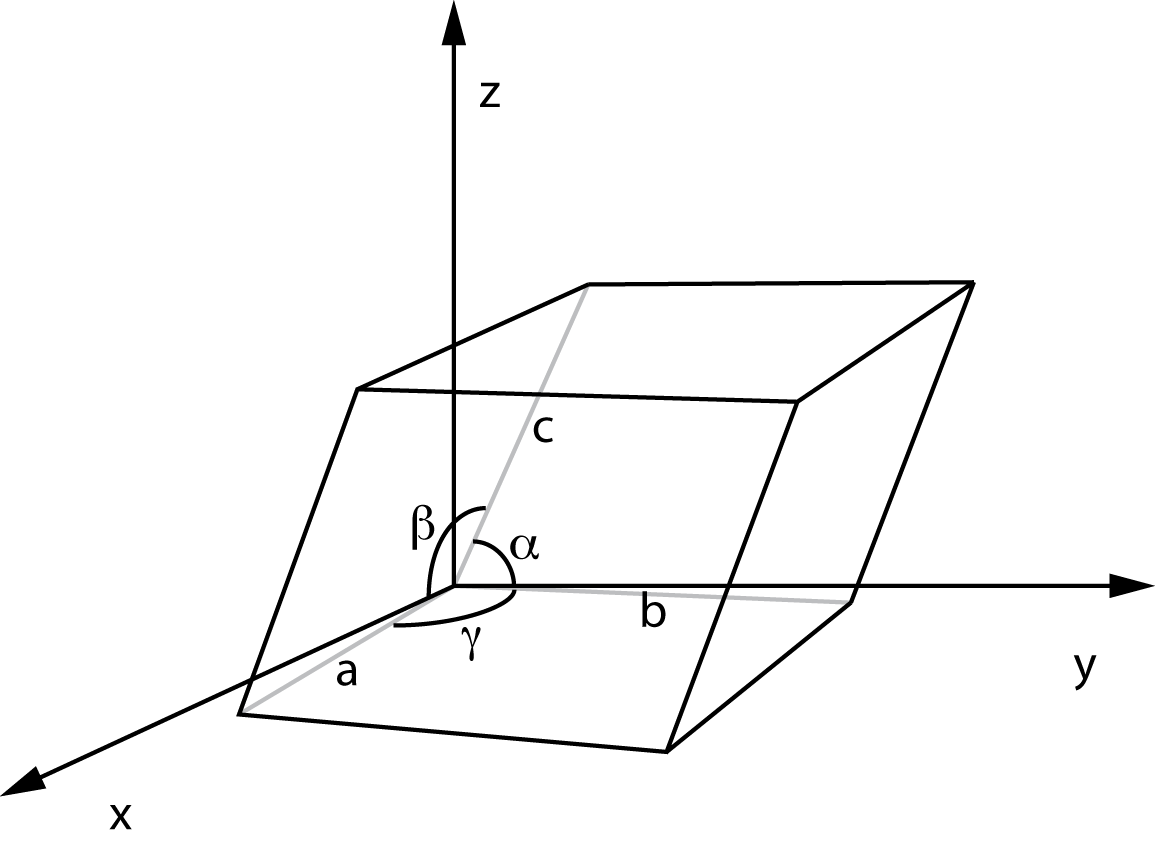
\includegraphics[scale=0.5]{../images/UnitCell.png}
\caption{Visual depiction of a unit cell. The coordinates of the atoms within the unit cell are given relative to the origin and the $a,b,c$ axes.}
\label{fig:Unit-Cell}
\end{figure}

\subsubsection{Average Properties Representation}
Our next representation uses a \textbf{16-element vector}, where each component is the mean of some atomic property over all of the atoms in that material, based on its reduced chemical formula. Our vector contained the following atomic properties:
{\small
\begin{tabular}{llll}
    Atomic volume & Atomic weight & Boiling point \\
    Covalent radius & Density & Electron affinity \\ 
    Electronegativity & Period table group & Heat of formation \\
    Heat of fusion & Heat of evaporation & Lattice constant\\
    Melting point & Period & Polarizability\\
    \multicolumn{2}{l}{Specific Heat at $T=20^\circ C$}
\end{tabular}}
Properties of atoms without a value for that property were given values of 0. Properties of materials without a value for that property - if, for example, all atoms in the material lack that property - were assigned a value equal to the average property value across all materials. We utilized this method to prevent such datapoints from skewing our classifier in an undesirable way.

\subsubsection{Combined Representation}
Our third representation is the concatenation of the unit-cell vector and the average properties vector, resulting in am \textbf{87-element vector} for each material.

\subsection{Emittance Labels}

For each material, we defined its minimum emittance as the lowest \textit{nonzero} emittance value (rounded to the nearest tenth to account for the $\pm0.05$ error from the calculations) achieved across at least two consecutive incident energies. Finally, we assigned a score of \textbf{one} to examples with minimum emittance \textbf{less than or equal to 0.2}, and a score of \textbf{zero} to those \textbf{greater than 0.2}. Figure \ref{fig:emittance-calc} illustrates the process by which labels were determined.

Our labelled dataset contained \textbf{3276} positive examples and \textbf{6160} negative examples for a total of 9436 materials. We randomly shuffled the data and performed a \textbf{80/10/10} train/validation/test split. The training set contained \textbf{2577} positive and \textbf{4971} negative examples.

\begin{figure}[ht]
\centering
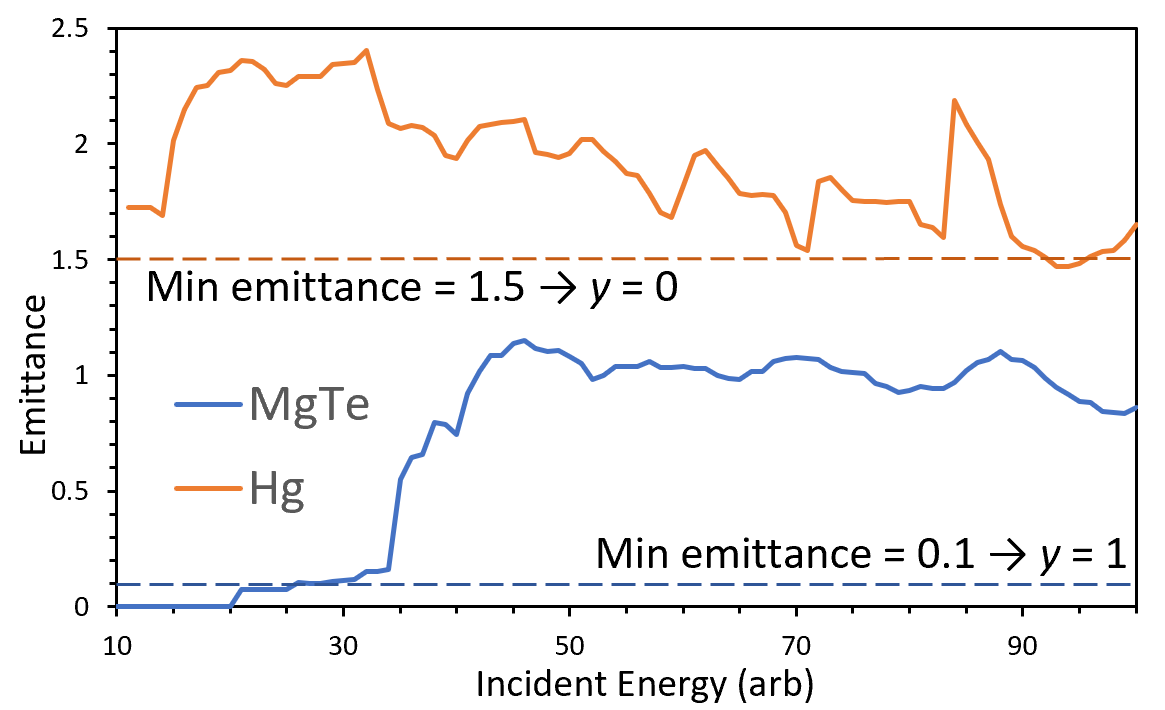
\includegraphics[width=\linewidth]{../images/emittance-plots.PNG}
\caption{Example visualization of emittance data for Magnesium Telluride and Mercury and their resulting labels, $y = 0$ and $y = 1$, respectively.}
\label{fig:emittance-calc}
\end{figure}

%%%%%%%%%%%%%%%%%% Methods %%%%%%%%%%%%%%%%%%%%%%%%%%%%%%%%%%%5
\section{Methodology}

Our project evaluated a number of different machine learning techniques, including both traditional and deep learning models, to determine the best model for this classification task. Each model was tuned on each of our different data representations. This section describes each model, as well as the techniques used for model evaluation.

\subsection{Traditional ML Techniques}

As part of our investigation of this data, we employed several traditional machine learning techniques. We implemented each classifier using its sklearn module. The models and hyperparameters deployed are as follows:
\begin{itemize}
    \item Logistic Regression - $L_2$ norm, $10^7$ iterations max
    \item SVM - penalty of 1.0, RBF kernel, kernel coefficient of $1/{\text{num features}}$
    \item Naive Bayes - Bernoulli model, no Laplace smoothing
    \item Random Forest - 100 trees, Gini impurity criterion
    \item K-Nearest Neighbors - $k = 2$, neighbors weighted by inverse of distance
\end{itemize}

\subsection{Neural Network}

In addition to the traditional ML models described above, we experimented with different fully-connected neural network models, adjusting hyperparameters such as the learning rate, number of epochs, number of hidden layers, and layer sizes. The neural network implementation we used is the sklearn Multilayer Perceptron Classifier class. Our best model across any data representation contains \textbf{7} hidden layers of sizes \textbf{(64, 128, 256, 512, 256, 128, 64)}, each followed by a \textbf{ReLU} nonlinearity. We used a learning rate of \textbf{0.0008}, the \textbf{binary cross entropy} (BCE) loss function, an L2 regularization parameter of \textbf{0.0001}, and an \textbf{Adam} optimizer to train the model.

\subsection{Evaluation Metrics}

Due to the asymmetry in our positive and negative examples, we knew that a simple accuracy metric would be insufficient to evaluate the performance of our model. We employed the following four metrics to evaluate model performance: \textbf{accuracy} ($acc$), \textbf{precision} ($pr$), \textbf{recall} ($re$), and \textbf{F1 score} ($f1$). Given the asymmetric label frequency in our dataset, the the $f1$ score is a better balanced metric than straight $acc$ to evaluate the model both on $pr$ and $re$. Our metrics are calculated using the following formulae:
$$acc = \frac{\text{True Pos + True Neg}}{\text{True Pos + True Neg + False Pos + False Neg}}$$
$$pr = \frac{\text{True Pos}}{\text{True Pos + False Pos}} $$
$$re = \frac{\text{True Pos}}{\text{True Pos + False Neg}}$$
$$f1 = \frac{2 * pr * re}{pr + re}$$

%%%%%%%%%%%%% Results + Discussion %%%%%%%%%%%%%%%%%%%%%%%%%%%%
\section{Results and Discussion}
\subsection{Results of Learning Methods on Validation Set}
\subsubsection{Unit Cell Representation}
\begin{center}
\begin{tabular}{|c|c|c|c|c|}
    \hline
    \textbf{Method} & \textbf{\textit{acc}} & \textbf{\textit{pr}} & \textbf{\textit{re}} & \textbf{\textit{f}1} \\
    \hline
    LogReg & 0.626 & 0.064 & 0.106 & 0.080 \\
    \hline
    SVM & 0.674 & 0.105 & 0.188 & 0.135 \\
    \hline
    NB & 0.552 & 0.230 & 0.336 & 0.273 \\
    \hline
    RF & 0.733 & 0.218 & 0.423 & 0.287 \\
    \hline
    kNN & 0.686 & 0.302 & 0.549 & 0.390 \\
    \hline
    NN & 0.668 & 0.331 & 0.585 & 0.423 \\
    \hline
\end{tabular}
\end{center}

\subsubsection{Average Properties Representation}
\begin{center}
\begin{tabular}{|c|c|c|c|c|}
    \hline
    \textbf{Method} & \textbf{\textit{acc}} & \textbf{\textit{pr}} & \textbf{\textit{re}} & \textbf{\textit{f}1} \\
    \hline
    LogReg & 0.639 & 0.081 & 0.137 & 0.102 \\
    \hline
    SVM & 0.685 & 0.130 & 0.235 & 0.167 \\
    \hline
    NB & 0.622 & 0.0 & 0.0 & N/A \\
    \hline
    RF & 0.749 & 0.273 & 0.541 & 0.363 \\
    \hline
    kNN & 0.676 & 0.268 & 0.479 & 0.344 \\
    \hline
    NN & 0.748 & 0.333 & 0.658 & 0.442 \\
    \hline
\end{tabular}
\end{center}

\subsubsection{Combined Representation}
\begin{center}
\begin{tabular}{|c|c|c|c|c|}
    \hline
    \textbf{Method} & \textbf{\textit{acc}} & \textbf{\textit{pr}} & \textbf{\textit{re}} & \textbf{\textit{f}1} \\
    \hline
    LogReg & 0.667 & 0.162 & 0.286 & 0.207 \\
    \hline
    SVM & 0.642 & 0.036 & 0.062 & 0.046 \\
    \hline
    NB & 0.551 & 0.231 & 0.336 & 0.274 \\
    \hline
    RF & 0.758 & 0.237 & 0.476 & 0.317 \\
    \hline
    kNN & 0.708 & 0.302 & 0.566 & 0.394 \\
    \hline
    NN & 0.734 & 0.330 & 0.641 & 0.436 \\
    \hline
\end{tabular}    
\end{center}

\subsection{Comparison of Learning Methods}
For each method, the neural net largely outperforms other methods, especially with the Average Properties and Combined representations. While the random forest achieved slightly higher accuracy across representations, the neural net was significantly superior in the other three metrics. Notably, the neural network achieved a higher $f1$ score, which we explained above provides a better measure of performance given the nature of our dataset. On the test set, the neural net with Average Properties gave the following results:
\begin{center}
\begin{tabular}{|c|c|c|c|c|}
    \hline
    \textbf{Model} & \textbf{\textit{acc}} & \textbf{\textit{pr}} & \textbf{\textit{re}} & \textbf{\textit{f}1} \\
    \hline
    NN w/ AvgPropRep & 0.701 & 0.296 & 0.573 & 0.390 \\
    \hline
\end{tabular}    
\end{center}

\subsection{Bias and Variance Analysis}
To analyze the efficacy of our neural net, we plot our training and cross-validation accuracies against number of training examples. We find that our model achieves greater than 90\% accuracy on the training dataset and much lower accuracy in the cross-validation, which shows that our model overfits our dataset and that regularization may improve the neural network model. We regularized our model with $\mathcal{L}_2$ regularization, testing weights between 0.01 and 0.9, but regularization did not significantly improve model performance, nor did it have much of an impact on the training accuracy, which suggests that regularization is not enough to combat the overfitting occuring in our model.

\begin{figure}[ht]
\centering
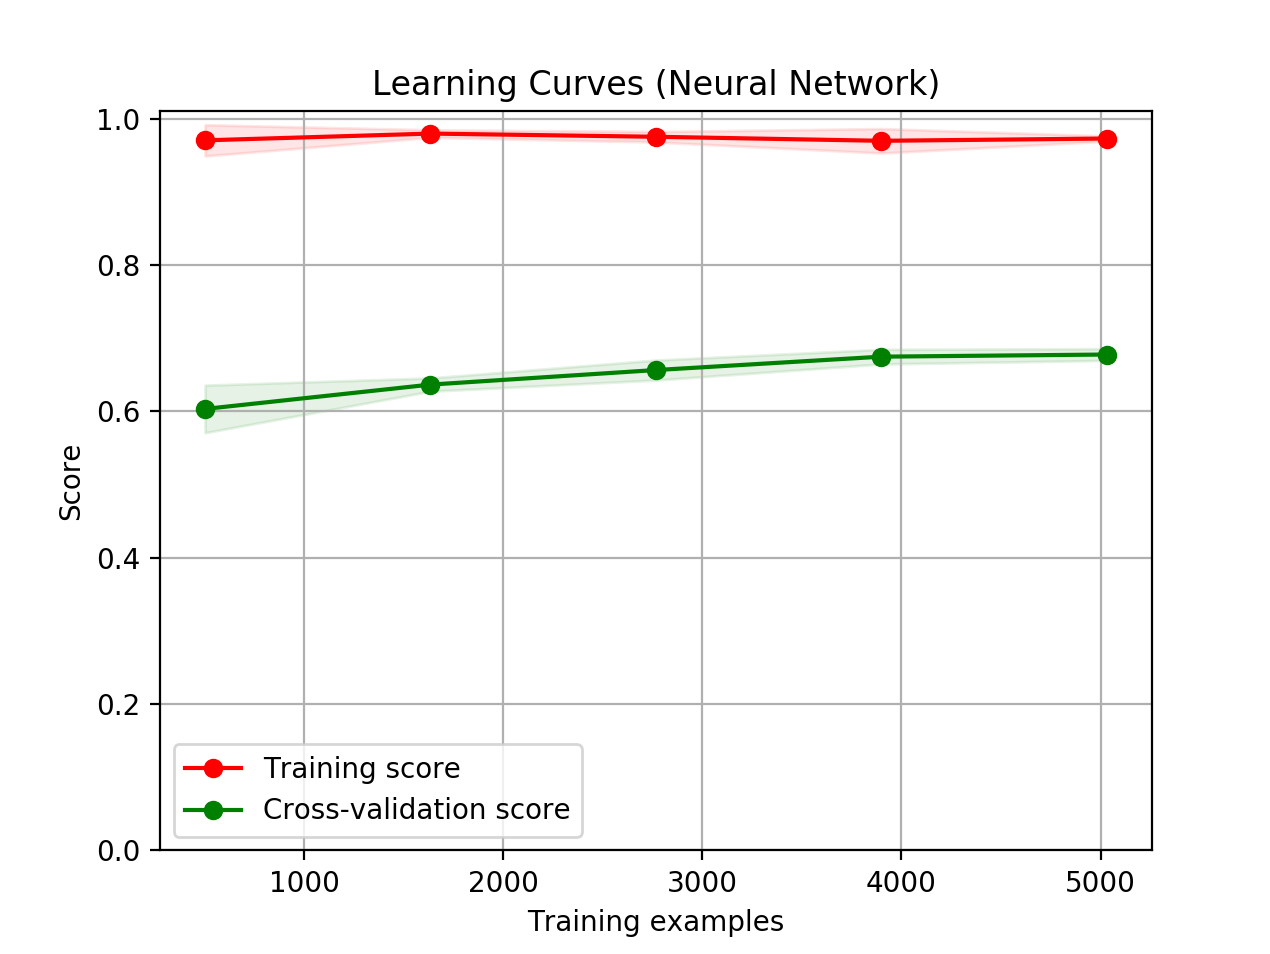
\includegraphics[width=\linewidth]{../images/LearningCurves.png}
\caption{Training and cross-validation learning curves for our seven-layer neural net with Average Properties representation (unregularized).}
\label{fig:emittance-calc}
\end{figure}

%%%%% DISCUSSION
\subsection{Discussion}

Our work demonstrates that it is possible to classify emittances with a greater than 70\% degree of accuracy using machine learning. We demonstrate that classification via machine learning is significantly faster than the DFT method: while DFT takes hours to days per material, our neural network predicts the emittance classification of one material in less than a second. The neural network model that we demonstrate, though, is an imperfect substitute for DFT; while DFT is able to calculate the exact emittance every time, we obtain a test set $f1$ score of 0.39. The more rapid classification provided by our system, though, provides a strong starting point for materials science research: researchers could, perhaps, employ our system to narrow a broad field of candidate materials, then run DFT on the most promising candidates.

We hypothesize several reasons as to why our system is unable to obtain a level of performance to rival DFT. First, observe the complex, multistep nature of the learning problem: we are asking the machine learning model to do the equivalent of generate the emittance vs. incident energy graph (Fig. 2), then minimize the graph. Generating the graph is a significant challenge in itself: the electronic band structure, and thus the emittance graph, can vary substantially based on minor changes to the input features. Second, perhaps a model with more data would perform better. The cross-validation curve (Fig. 3) increases over with the number of training examples, which suggest that adding more data would improve performance. We conjecture that our 9,436-point dataset, though substantial, may be too small for our neural net to comprehensively establish the impact of the value of each feature on the overall emittance classification (this may be why our neural network performed best on the average properties representation, which contained the fewest features). Thirdly, there is room for improvement in our data representation; below, we compare our material representation models one-by-one.

\subsection{Discussion of Representation Methods}
\subsubsection{Unit Cell Representation}
The main strength of the unit cell representation is that it encodes the structure of the material. The unit cell representation is an encoding of the entire input of DFT calculations. Theoretically, it thus encodes all of the information needed to predict emittance. However, the unit cell representation suffers from inconsistent vector lengths, as not all materials will have the same number of atoms in their unit cells. To address this, we truncated all vectors to represent up to 16 atoms and padded with zeros wherever needed; this may have brought about unintended consequences in our training. 

Another shortcoming of the unit cell representation is that each material does \textit{not} have many different encodings.   In particular, the feature vector could have its component atoms reordered and still represent the same material, or the origin of the unit cell could be made to start at a different position relative to its atoms, such that all of the coordinates end up being translated by some amount; such a change would still result in the same material. A third drawback of the unit cell representation is that it fails to successfully capture the relationships between atoms in the material. By merely listing the identities and positions of the atoms, the unit cell representation does not capture which atoms are bonded to each other, the quantity and arrangement of each atom's nearest neighbors, the identities of those nearest neighbors, among others.

\subsubsection{Average Properties Representation}
The main strength of this representation is that a feature vector can be generated for any material, as long as its chemical composition is known. Thus, even materials that have never been synthesized can be easily represented. The use of a fixed list of properties also more successfully standardizes the length of each vector. However, due to the wide variety of compounds in our dataset, not all information is available for all elements in \texttt{mendeleev}, so this representation still requires padding to some degree. Furthermore, many different materials can have the same composition, which would result in identical feature vectors. 

Perhaps the main weakness of the average properties representation is that it loses explicit structural/ crystallographic information about the material, which means the link between materials properties and emittances, which are derived from the output of DFT calculations, is quite indirect. Perhaps this explains why the neural net outperformed all of our other learning methods, as neural network architecture can somewhat compensate for the oblique link between our features and labels. It is possible that adding  more properties to our feature vectors would improve the performance of this method. 

Another potential avenue of improvement would be to include properties of the whole material, not just its atoms. This would allow the curation of features that, through physical or empirical models, are thought to correlate strongly with emittance, rather than just a wide variety of less-related atomic properties. However, there is still room for research into finding such features, and it is not guaranteed that such properties are already known for all materials being screened; this is especially true for materials for which we can not yet fabricate physical samples.


%%%%%%%%%%%%% Conclusions and Future Work %%%%%%%%%%%%%%%%%%%%%%%%%%%%
\section{Conclusions and Future Work}

In conclusion, our work shows that there is significant promise for machine learning to add valuable insight as a rapid-screening mechanism for materials science research.

The design of molecular representations for computational materials science is an active area of research, and future work may be able to build off of novel representations to achieve better performance. Promising representations for future study include the models implemented in \texttt{DScribe}, provided the input data is stratified to use the appropriate representation, as well as the MEGNet model described by Chen \textit{et al}, in which both molecules and crystals are encoded as graph networks \cite{MEGNet}.

In future work, decomposing our multistep classification problem into discrete steps, each modeled as a separate machine learning task, may prove fruitful. For example, machine learning may be applied to determine emission spectra (after which standard techniques are used to minimize the curve), or used to generate the atomic band structure (thereby supplanting DFT). The latter, though a lofty task, would be a significant step forward in the field of computational machine learning.

%%%%%%%%%%%%% Appendix %%%%%%%%%%%%%%%%%%%%%%%%%%%%
\section{Appendix}

Our Github repository can be found at \url{https://github.com/theCaiGuy/Photocathode-Materials}

%-------------------------------------------------------------------------
\section{Acknowledgements}
We would like to thank the Reed group both for inspiring this project and for being an incredible resource for us throughout. We would especially like to acknowledge Evan Antoniuk, a PhD student in the Reed group, who has been our primary contact throughout this process and provided us with both the dataset to make the project happen, and the knowledge to understand the task at hand.

Features for each material were extracted from the open-source Materials Project API and the \texttt{mendeleev} package. All model implementations were drawn from the open-source SciKit Learn package.


\section{Contributions}
Jennie Yang and Michael Cai worked on extracting and cleaning data for each material from an online database. Jennie also took care of the literature review and other areas of the project that required materials science background.

Michael Cooper and Jennie Yang built the traditional machine learning models (log reg, NB, SVM, random forest), while Michael Cai built and fine-tuned the neural network. All group members contributed to running the models across different representations, compiling performance data, and debugging issues with our implementations and dataset.

All three group members contributed equally to the poster and project writeup.

%-------------------------------------------------------------------------
% \section{References}

{\small
\bibliographystyle{ieee_fullname}

\begin{thebibliography}{7}
\bibitem{Dowell}
D. H. Dowell \textit{et al}, “Cathode R\&D for Future Light Sources,” \textit{Nuclear Instruments and Methods in Physics Research Section A}, vol. 622, no. 3, pp. 685–697, Oct. 2010.

\bibitem{Bazarov}
I. Bazarov \textit{et al}, "Thermal emittance measurements of a cesium potassium antimonide photocathode," \textit{Applied Physics Letters}, vol. 98, 02 Jun. 2011.

\bibitem{Li}
T. Li \textit{et al}, "Emission properties of body-centered cubic elemental metal photocathodes," \textit{Journal of Applied Physics}, vol. 117, 10 Mar. 2015.

\bibitem{DScribe}
L. Himanen \textit{et al}, "DScribe: Library of Descriptors for Machine Learning in Materials Science," \texttt{arXiv:1904.08875 [cond-mat.mtrl-sci]}, 18, Apr. 2019. 

\bibitem{Cubuk}
E. Cubuk, \textit{et al} "Screening billions of candidates for solid lithium-ion conductors: A transfer learning approach for small data" \textit{Journal of Chemical Physics}, vol 150, 3 Jun. 2019.

\bibitem{MEGNet}
C. Chen \textit{et al}, "Graph Networks as a Universal Machine Learning
Framework for Molecules and Crystals," \texttt{arXiv:1812.05055v2 [cond-mat.mtrl-sci]}, 28 Feb. 2019.

\bibitem{mendeleev}
L. M. Mentel, \texttt{mendeleev} - A Python resource for properties of chemical elements, ions and isotopes, 2014.

\end{thebibliography}


}
\end{document}
